\documentclass[tikz, border=3mm]{standalone}
\usepackage{tikz}
\usetikzlibrary{arrows.meta, positioning}

\begin{document}
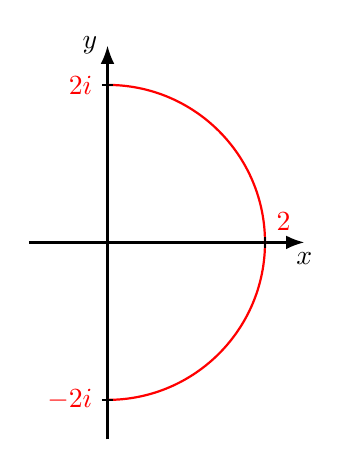
\begin{tikzpicture}[
    >=Latex, % Set default arrow tip style
    axis/.style={->, thick}, % Style for axes
    pathstyle/.style={red, thick}, % Style for the semi-circular path
    labelstyle/.style={red}, % Style for labels
    tick/.style={thick} % Style for tick marks
]

    % Axes
    \draw[axis] (-1, 0) -- (2.5, 0) node[below] {$x$}; % x-axis
    \draw[axis] (0, -2.5) -- (0, 2.5) node[left] {$y$}; % y-axis

    % Define Key Points (intersections with axes)
    \coordinate (Top)    at (0, 2);  % Top point on y-axis
    \coordinate (Bottom) at (0, -2); % Bottom point on y-axis
    \coordinate (Right)  at (2, 0);  % Rightmost point on x-axis
    \def\radius{2} % Radius of the circle

    % Draw the red semi-circular arc
    % Start at Top (angle 90), end at Bottom (angle -90), radius 2
    \draw[pathstyle] (Top) arc (90:-90:\radius);

    % Ticks at intersection points
    \draw[tick] (-2pt, 2) -- (2pt, 2);  % Tick at y=2
    \draw[tick] (-2pt, -2) -- (2pt, -2); % Tick at y=-2
    \draw[tick] (2, -2pt) -- (2, 2pt);  % Tick at x=2

    % Labels for the ticks
    \node[labelstyle, left=2pt] at (Top) {$2i$};
    \node[labelstyle, left=2pt] at (Bottom) {$-2i$};
    \node[labelstyle, above right=1pt] at (Right) {$2$};

\end{tikzpicture}
\end{document}